\section{Módulo de Integração}
\label{sec:modulo-integracao}

	O Módulo de Integração é responsável pela integração do Sistema TRUE  com o
	Middleware \textit{uOS}. Através desta integração, os dados providos pelo Sistema TRUE (localização
	e identificação dos usuários em um ambiente) são disponibilizadas ao ambiente gerenciado pelo middleware \textit{uOS}
	por meio de serviços. Para integrá-los foi desenvolvido um \textit{driver} para o Middleware se comunicar
	com o Sistema TRUE. Este \textit{driver} foi nomeado de \textit{UserDriver} cujo diagrama de classe
	é mostrado na Figura~\ref{fig:userdriver}. A integração foi feita utilizando
	suporte JNI (\textit{Java Native Interface} - Apêndice~\ref{apend:jni}) uma vez que o Middleware foi desenvolvido em JAVA e o Sistema TRUE em C++.

	% O Módulo de Integração é responsável pela integração do Sistema TRUE  com o
	% Middleware \textit{uOS}. Os dados providos pelo Sistema TRUE (localização
	% e identificação dos usuários em um ambiente) são informações de
	% contexto relevantes para ambientes inteligentes. O Middleware \textit{uOS} foi
	% escolhido como meio de fornecê-las as diversas aplicações no ambiente. Então,
	% para integrá-los foi desenvolvido um \textit{driver} para o Middleware se comunicar
	% com o Sistema TRUE. Este \textit{driver} foi nomeado de \textit{UserDriver} cujo diagrama de classe
	% é mostrado na Figura~\ref{fig:userdriver}. A integração foi feita utilizando
	% suporte JNI (\textit{Java Native Interface} - Apêndice~\ref{apend:jni}) uma vez que o Middleware foi desenvolvido em JAVA e o Sistema TRUE em C++.

	\begin{figure}[htb]
		\begin{center}
			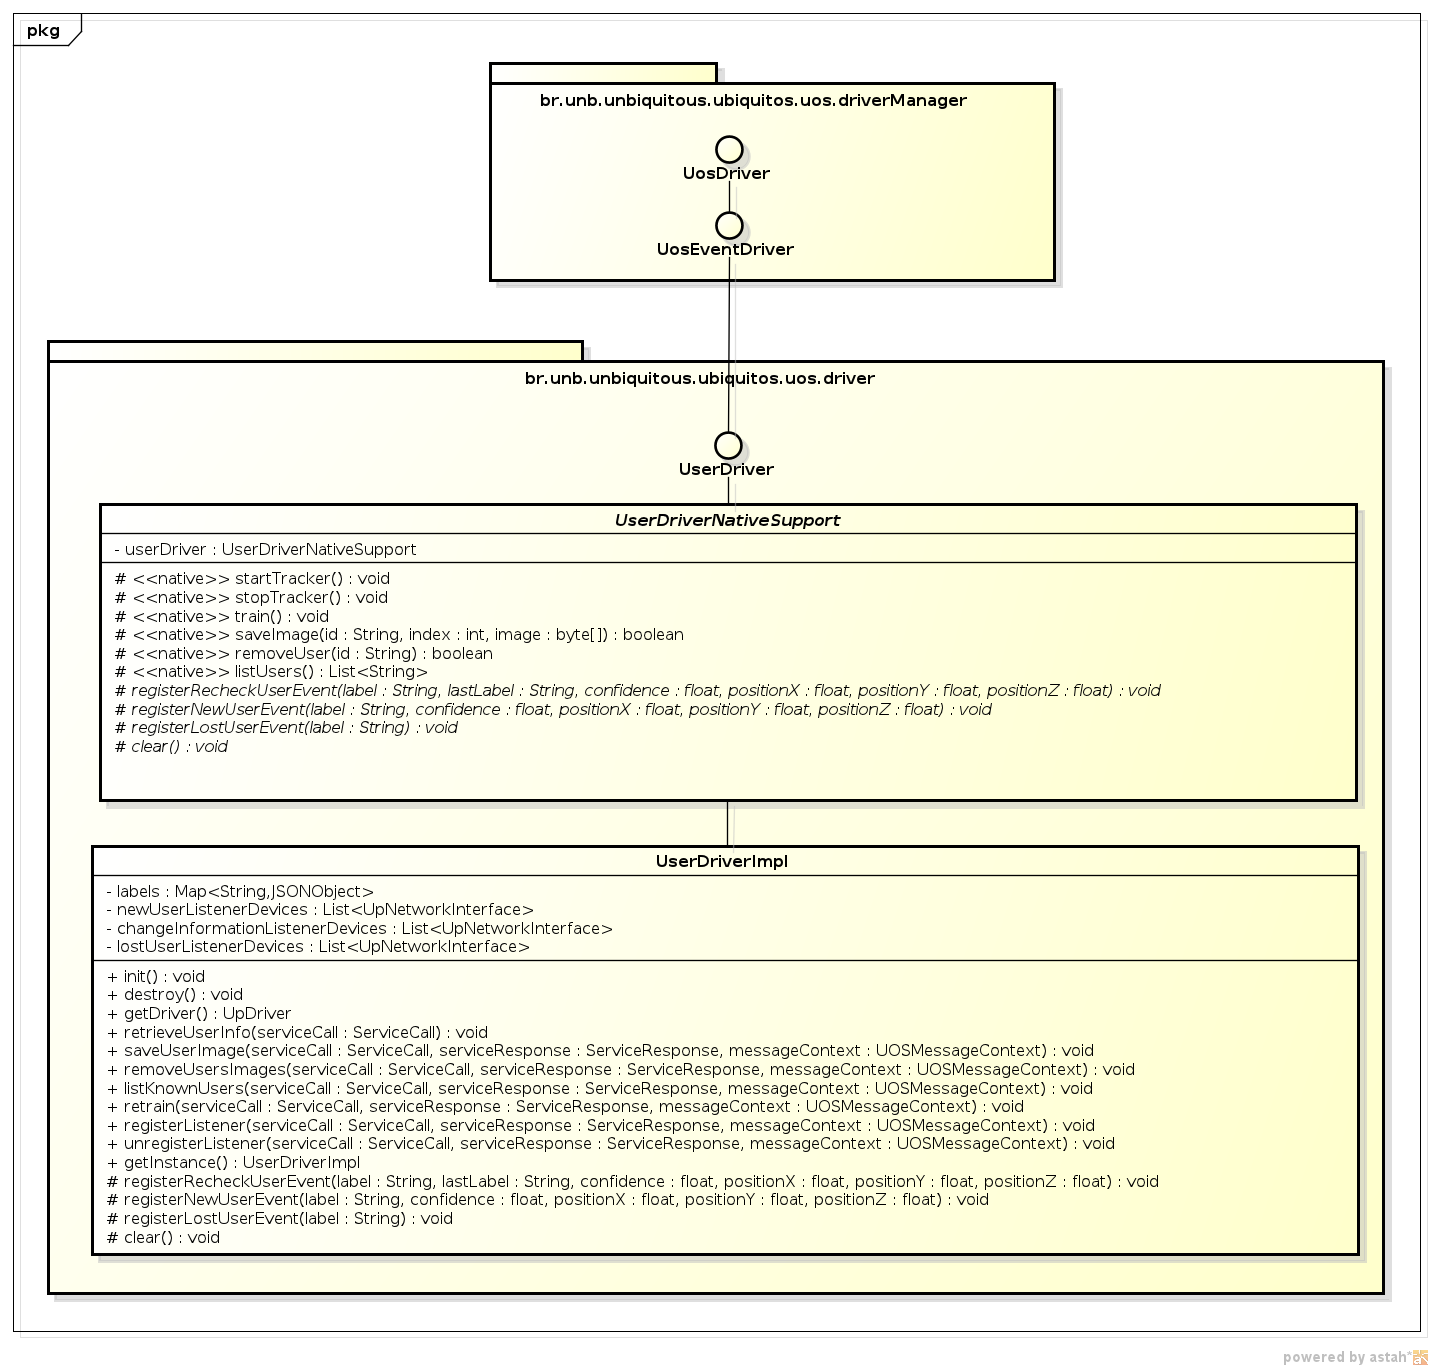
\includegraphics[scale=0.45]{figuras/4.ProblemaEProposta/diagrama-classe-userdriver.png}
		\end{center}
		\caption{Diagrama de Classe do UserDriver.}
		\label{fig:userdriver}
	\end{figure}

Os métodos do \textit{UserDriver} podem ser divididos basicamente em três grupos, isto é, métodos de inicialização, métodos nativos e de serviços e eventos:

\begin{itemize}
	\item \textbf{Métodos de Inicialização}: métodos responsáveis pela inicialização do Sistema TRUE e pelo registro dos serviços que o \textit{driver} possui e os eventos que pode gerar.

	\item \textbf{Métodos Nativos}: métodos declarados no \textit{driver} que permitem acessar alguns métodos implementados pelo Sistema TRUE. Tais métodos permitem que o \textit{UserDriver} tenha controle sobre o sistema, podendo iniciá-lo, encerrá-lo, retreiná-lo e, até mesmo, cadastrar e remover novos usuários a qualquer momento. Para implementar os métodos nativos foi utilizado JNI (\textit{Java Native Interface}), descrito no Apêndice~\ref{apend:jni}.

	\item \textbf{Serviços e Eventos}: são os métodos que implementam os serviços que o \textit{UserDriver} disponibiliza às aplicações presentes no ambiente e os eventos que pode gerar. 

	% Nestes serviços incluem consultas as informações (nome e localização) de qualquer usuário presente no ambiente, listagem dos usuários no ambiente, cadastro e remoção de novos usuário do Sistema TRUE e retreino do mesmo, e registro de \textit{listeners} que ``escutam'' os eventos gerados pelo driver. Nos eventos incluem evento de um novo usuário detectado, evento de um usuário perdido, evento de quando a identidade do usuário é corrigida e um outro evento que é gerado de tempo em tempo atualizando a posição de todos os usuários no ambiente.

\end{itemize}



	O \textit{UserDriver} disponibiliza às aplicações registradas no
	\textit{middleware} os seguintes serviços:

	\begin{itemize}
		\item \textbf{Consultas as informações dos usuários no ambiente}: através dessas consultas, as aplicações tem acesso ao nomes, emails, posições correntes e confiança do reconhecimento de todos os usuários presentes no ambiente.
		\item \textbf{Cadastro}: as aplicações podem cadastrar novos usuários fornecendo ao \textit{UserDriver} o nome, o email e as imagens do novo usuário.
		\item \textbf{Treino do sistema}: após cadastrar novos usuários as aplicações podem retreinar o sistema para poder reconhecer o novo usuário cadastrado.
		\item \textbf{Remoção}: as aplicações podem remover usuários cadastrados fornecendo o email do usuário.
		\item \textbf{Registro de \textit{listeners}}: as aplicações podem registrar \textit{listeners} para ``escutar'' os eventos gerados pelo \textit{UserDriver}.
	\end{itemize}

Além dos serviços, o \textit{UserDriver} gera os seguintes eventos:

	\begin{itemize}
		\item \textbf{Novo Usuário}: evento gerado assim que um novo usuário foi detectado pelo Sistema TRUE.
		\item \textbf{Usuário Perdido}: evento gerado assim que um usuário deixou de ser rastreado pelo Sistema TRUE.
		\item \textbf{Atualização dos dados do usuário}: evento gerado a cada cinco segundos atualizando os dados de todos os usuários rastreados.
	\end{itemize}

	O Módulo de Integração se comunica diretamente com os Módulos de Rastreamento e de
	Registro através do \textit{UserDriver}. Enquanto a comunicação com o Módulo de
	Registro acontece somente quando alguma aplicação solicita o cadastramento ou a remoção
	de usuários, a comunicação com o Módulo de Rastreamento acontece constantemente:

	\begin{itemize}
		\item a cada 5 segundos o Módulo de Rastreamento envia informações correntes sobre todos os usuários no ambiente atualizando as informações que o Módulo de Integração detém;
		\item sempre que um usuário entra ou sai do ambiente o Módulo de Rastreamento informa o Módulo de Integração.
	\end{itemize} 

	Através do \textit{UserDriver}, o Middleware \textit{uOS} tem acesso às
	informações sobre identidade e localização dos usuários presentes no ambiente em
	tempo real. Tais informações ficam disponíveis a qualquer aplicação registrada
	no Middleware.
